%\documentclass[12pt]{article}
%\usepackage[a4paper, margin=1in]{geometry} 
%\usepackage{graphicx} 
%\usepackage{hyperref}
%\usepackage{float}
%\usepackage{multicol}
%\usepackage{amsmath}
%\usepackage[ruled]{algorithm2e}
%\usepackage{amssymb}
%\usepackage[font=small, labelfont=bf]{caption}

%\begin{document}

%
% Backtracking
%
\subsection{Backtracking}
Backtracking is a post-processing procedure to find the alignments that have yielded the best score. 

%
% Store movement in cells
%
\subsubsection*{Store movement in cells}

A table cell can be used for storing the movement.
\begin{figure}[H]
  \centering
      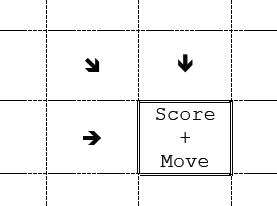
\includegraphics[width=0.3\textwidth]{fig02/back_tracking_store_moves.png}
\end{figure}

\noindent \textbf{Example}
\begin{multicols}{2}
Cells with scores and directions
\begin{figure}[H]
  \centering
      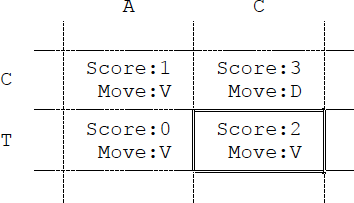
\includegraphics[width=0.3\textwidth]{fig02/back_tracking_store_moves_example.png}
\end{figure}

Use arrows to indicate backtracking
\begin{figure}[H]
  \centering
      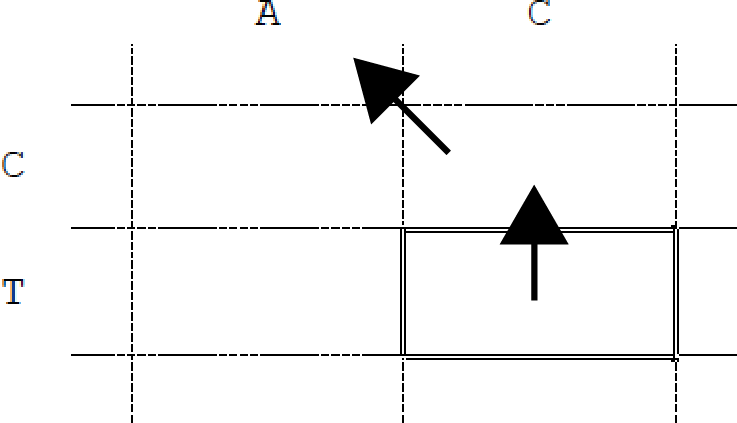
\includegraphics[width=0.3\textwidth]{fig02/back_tracking_store_moves_arrows.png}
\end{figure}

\end{multicols} 

%
% Exercise \thesection.6
%
\subsubsection*{Exercise \thesection.6}
	
Complete the DP table with scores and directions. What is the alignment with the best score?

\begin{multicols}{2}
\begin{figure}[H]
  \centering
      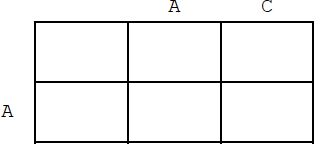
\includegraphics[width=0.3\textwidth]{fig02/back_tracking_store_moves_exercise.png}
\end{figure}

\noindent Scoring scheme: \\ 
$R_{ab}$ = 1 for a = b \\ 
$R_{ab}$ = 0 for a $\neq$ b \\ 
g = 1

\end{multicols} 

%
% Re-calculate candidate scores
%
\subsubsection*{Re-calculate candidate scores}

Re-calculating the three candidate scores also reveals the movement.

\begin{align*}
H_{i,j}^{(0)} &= H_{i-1,j} - g &(vertical) \\
H_{i,j}^{(1)} &= H_{i,j-1} - g &(horizontal) \\
H_{i,j}^{(2)} &= H_{i-1,j-1} + R_{a,b} &(diagonal)
\end{align*}

\noindent \textbf{Example}

\begin{figure}[H]
  \centering
      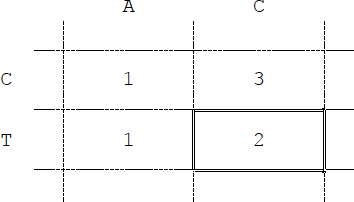
\includegraphics[width=0.3\textwidth]{fig02/back_tracking_example.png}
\end{figure}
				
\begin{align*}
H_{i,j}^{(0)} &= 3 - 1 = 2 = H_{i,j} &\checkmark & (vertical) \\
H_{i,j}^{(1)} &= 1 - 1 = 0 \neq H_{i,j} &\hfill & (horizontal) \\
H_{i,j}^{(2)} &= 1 + 0 = 1 \neq H_{i,j} &\hfill  & (diagonal)
\end{align*}

%
% Common mistake with backtracking
%
\subsubsection*{Common mistake with backtracking}
For the re-calulation approach, it is not to find $max(H_{i-1,j}, H_{i,j-1}, H_{i-1,j-1})$. You must re-calulate the candidates and then $max(H_{i,j}^{(0)}, H_{i,j}^{(1)} , H_{i,j}^{(2)})$ to find the actual direction.

%
% Implementation with recursive call
%
\subsubsection*{Implementation with recursive call}
Recursive calls are usually used to implement DP backtracking.

\begin{algorithm}[H]
  \SetKwInOut{HAB}{$\mathrm{H_{i,j}}$}
  \SetKwInOut{RAB}{$\mathrm{R_{a,b}}$}
  \SetKwInOut{G}{$\mathrm{g}$}
  
  \SetKwProg{Fn}{proc}{}{end}
  \SetKwInOut{I}{$\mathrm{i}$}
  \SetKwInOut{J}{$\mathrm{j}$}
  \SetKwInOut{SQ}{$\mathrm{S_{q}}$}
  \SetKwInOut{SD}{$\mathrm{S_{d}}$}
  \SetKwInOut{AQ}{$\mathrm{A_{q}}$}
  \SetKwInOut{AD}{$\mathrm{A_{d}}$}
  \SetKwInOut{K}{$\mathrm{k}$}

  \SetKwData{dI}{$\mathrm{i}$}
  \SetKwData{dJ}{$\mathrm{j}$}
  \SetKwData{dAQ}{$\mathrm{A_{q}}$}
  \SetKwData{dAD}{$\mathrm{A_{d}}$}
  \SetKwData{dK}{$\mathrm{k}$}
    
  \SetKwData{dRAB}{$\mathrm{R_{a,b}}$}
  \SetKwData{dG}{$\mathrm{g}$}

  \BlankLine
  
  \SQ{Sequence q}
  \SD{Sequence d}     
  \HAB{Dyanamic programming table}
  \RAB{Match/mismatch scores}
  \G{Gap penalty}

  \BlankLine \BlankLine

  \Fn{backTrack(\dI, \dJ, \dAQ, \dAD, \dK)}{
    
    \BlankLine
    
    \I{Index of sequence q}
    \J{Index of sequence d}
    \AQ{q part of alignement (stored in reverse order)}
    \AD{d part of alignement (stored in reverse order)}
    \K{Index for \dAQ and \dAD}
  
    \BlankLine
    
    \tcp{}
    \tcp{Need to implement recursion termination here}
    \tcp{...}
    \tcp{}
        
    \BlankLine
    
    \If(\tcp*[f]{vertical}){$\mathrm{H_{i,j}} = \mathrm{H_{i-1,j}} - g$}{
      $\mathrm{A_{q, k}} $ $\leftarrow$ $ S_{q, i}$\;
      $\mathrm{A_{d, k}} $ $\leftarrow$ $ $ '-'\;
      $backTrack$($\mathrm{i-1}$, \dJ, \dAQ, \dAD, $k + 1$)\;
    }
    \BlankLine

    \If(\tcp*[f]{horizontal}){$\mathrm{H_{i,j}} = \mathrm{H_{i,j-1}} - g$}{
      $\mathrm{A_{q, k}} $ $\leftarrow$ '-'\;
      $\mathrm{A_{d, k}} $ $\leftarrow$ $ S_{d, i}$\;
      $backTrack$(\dI, $\mathrm{j-1}$, \dAQ, \dAD, $k + 1$)\;
    }
    \BlankLine
    
    \If(\tcp*[f]{diagonal}){$\mathrm{H_{i,j}} = \mathrm{H_{i-1,j-1}} +\mathrm{R_{S_{q, i},S_{d, i}}}$}{
      $\mathrm{A_{q, k}} $ $\leftarrow$ $ S_{q, i}$\;
      $\mathrm{A_{d, k}} $ $\leftarrow$ $ S_{d, i}$\;
      $backTrack$($\mathrm{i-1}$, $\mathrm{j-1}$, \dAQ, \dAD, $k + 1$)\;
    }
      
    \BlankLine
  }

  \SetAlgoRefName{\thesection.2}
  \caption{DP backtracking}

\end{algorithm}

%
% Exercise \thesection.7
%
\subsubsection*{Exercise \thesection.7}
	
Find the alignment with the best score.

\begin{multicols}{2}
\begin{figure}[H]
  \centering
      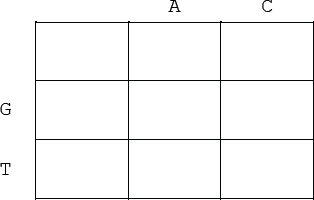
\includegraphics[width=0.3\textwidth]{fig02/back_tracking_exercise.png}
\end{figure}

\noindent Scoring scheme: \\ 
$R_{ab}$ = 1 for a = b \\ 
$R_{ab}$ = 0 for a $\neq$ b \\ 
g = 1

\end{multicols} 

%\end{document}
